%TODO! - Proper citations

%----------------------------------------------------------------------------------------
% PACKAGES AND OTHER DOCUMENT CONFIGURATIONS
%----------------------------------------------------------------------------------------

\documentclass[a4paper]{article}
\usepackage{fontspec}
\usepackage[autostyle]{csquotes}

% == Package includes
\usepackage[backend=biber, style=ieee]{biblatex}              % Biblatex with IEEE Config
  \addbibresource{references.bib}
\usepackage{booktabs}                                                    % Table support|
\usepackage[table]{xcolor}                                               %              |
%\usepackage[a4paper,bindingoffset=-0.1in,left=1in,right=1in,top=1in,bottom=1in,footskip=1in]{geometry}
\usepackage{fancyhdr}                                       % Required for custom headers
\usepackage[perpage, bottom]{footmisc}
\usepackage{lastpage}                % Required to determine the last page for the footer
\usepackage{extramarks}                                % Required for headers and footers
\usepackage{graphicx}                                         % Required to insert images
\usepackage{lipsum}       % Used for inserting dummy 'Lorem ipsum' text into the template
\usepackage[english]{babel}                                % English language/hyphenation
\usepackage{mathtools}                                                    % Math packages
\usepackage{mathabx}
%\usepackage{amsmath,amsfonts,amsthm}                        % Math packages (deprecated)
\usepackage{float}                                              % Images and other floats
\usepackage[section]{placeins}                                      % Placement of floats
\usepackage{color}                                                       % Colour support
\usepackage{tikz}
\usepackage{pgfplots}
  \pgfplotsset{compat=1.11}
\usepackage{chngcntr}                                           % Figure counter settings
\usepackage[hidelinks]{hyperref}                                             % Hyperlinks
\usepackage{epstopdf}                                               % EPS graphic support
\usepackage{pygmentex}                                       % Code snippet color support
\usepackage{listings}                                              % Code snippet support
\usepackage{minted}                                                       % Code snippets
\usepackage{bm}                                                      % Bold maths symbols
\usepackage{enumerate}                                                            % Lists


% == Colour Definitions
\definecolor{dkgreen}{rgb}{0,0.6,0}
\definecolor{gray}{rgb}{0.93,0.93,0.93}
\definecolor{mauve}{rgb}{0.58,0,0.82}

% == Code Snippet Config
\DeclareBoolOption[true]{cache}
\setmonofont{Consolas}
\usemintedstyle{friendly}
\setminted{bgcolor=gray, fontsize=\small}
\lstset{frame=tb,
  aboveskip=3mm,
  belowskip=3mm,
  showstringspaces=false,
  columns=flexible,
  basicstyle={\small\ttfamily},
  numbers=none,
  breaklines=true,
  breakatwhitespace=true
  tabsize=3
}


\providecommand{\e}[1]{\ensuremath{\times 10^{#1}}}                % Scientific Notation!
\providecommand{\eoc}{\ensuremath{_{\slash \slash \slash}}}           % End of Calculation Symbol!
%\flushbottom

%----------------------------------------------------------------------------------------
% DOCUMENT STRUCTURE COMMANDS
%----------------------------------------------------------------------------------------

% == Numbering

\makeatletter

\newcommand\frontmatter{%
    \cleardoublepage
  %\@mainmatterfalse
  \pagenumbering{roman}}

\newcommand\mainmatter{%
    \cleardoublepage
 % \@mainmattertrue
  \pagenumbering{arabic}}

\newcommand\backmatter{%
  \if@openright
    \cleardoublepage
  \else
    \clearpage
  \fi
 % \@mainmatterfalse
   }

\makeatother

% == Margins
\topmargin=-0.45in                                   % Deprecated due to geometry package
\evensidemargin=0in
\oddsidemargin=0in
\textwidth=6.5in
\textheight=10in
\headsep=0.25in
\setlength\parindent{0pt}                       % Removes all indentation from paragraphs
\linespread{1.1}                                                           % Line spacing

% == Header and Footer
\pagestyle{fancy}
\lhead{\footnotesize\reportAuthorName}                                    % Top left header
\chead{}                                                              % Top center header
\rhead{\firstxmark\reportClass\ | \reportTitle}                      % Top right header\first
\lfoot{\lastxmark}                                                   % Bottom left footer
\cfoot{}                                                           % Bottom center footer
\rfoot{Page\ \thepage}                                              % Bottom right footer
\renewcommand\headrulewidth{0.4pt}                              % Size of the header rule
\renewcommand\footrulewidth{0.3pt}                              % Size of the footer rule
                                                       % Custom preamble
%----------------------------------------------------------------------------------------
% NAME AND CLASS SECTION
%----------------------------------------------------------------------------------------

\newcommand{\hmwkTitle}{Project Report} % Assignment title
\newcommand{\hmwkDueDate}{Wednesday,\ September\ 03,\ 2014}                    % Due date
\newcommand{\hmwkClass}{EEE3061W - Mechatronics Design}                    % Course/class
\newcommand{\hmwkClassTime}{10:30am}                                 % Class/lecture time
\newcommand{\hmwkClassInstructor}{Jones}                               % Teacher/lecturer
\newcommand{\hmwkAuthorName}{WDXSEA003 \textbar \space PRSSAM004 \textbar \space RJDYAR001 \textbar \space STRIBR001}    % Your name
\newcommand{\hmwkDepartment}{Department of Electrical Engineering}           % Department

%----------------------------------------------------------------------------------------
% TITLE PAGE
%----------------------------------------------------------------------------------------

\title{
\begin{figure}[H]
  \begin{center}
    \includegraphics[width=0.4\columnwidth]{uct-logo}
  \end{center}
\end{figure}
\textmd{\Huge UNIVERSITY OF CAPETOWN \\ \LARGE \hmwkDepartment} \\
\vspace{2in}
\textmd{\textbf{\LARGE \hmwkClass\\ \Huge Biathlon Robot \\ \hmwkTitle \\ \vspace{1.5in} \Large Team 13 \\  \hmwkAuthorName}}\\
%\normalsize\vspace{0.1in}\small{Due\ on\ \hmwkDueDate}\\
%\vspace{0.1in}\large{\textit{\hmwkClassInstructor\ \hmwkClassTime}}
}

\date{}

%========================================================================================
%========================================================================================

\begin{document}

\maketitle
\clearpage

%----------------------------------------------------------------------------------------
% ABTRACT
%----------------------------------------------------------------------------------------
\setcounter{tocdepth}{2}                                                      % ToC Depth

\begin{abstract}
This report covers the design procedure and results for an active noise cancelling headset preamplifier which performed to the specified requirements when simulated and demonstrated reasonable noise cancelling characteristics.
\end{abstract}
% \newpage

%----------------------------------------------------------------------------------------
% TABLE OF CONTENTS
%----------------------------------------------------------------------------------------

\clearpage

\tableofcontents

\clearpage

\listoffigures
\listoftables

\clearpage

%----------------------------------------------------------------------------------------
% NOMENCLATURE
%----------------------------------------------------------------------------------------

\begin{homeworkProblem}[{Nomenclature}]
\textbf{Constants}

\(V_{LINE}\) - Nominal Line Voltage\\
\(A_v\) - Operational Amplifier Gain\\
\(db_{SPL}\) - Sound Pressure Level\\
\(\theta_S\) - Phase Shift

\end{homeworkProblem}
%----------------------------------------------------------------------------------------
% INTRODUCTION
%----------------------------------------------------------------------------------------
\begin{homeworkProblem}[{Introduction}]
% Graph:
\begin{figure}[H]
  \centering
  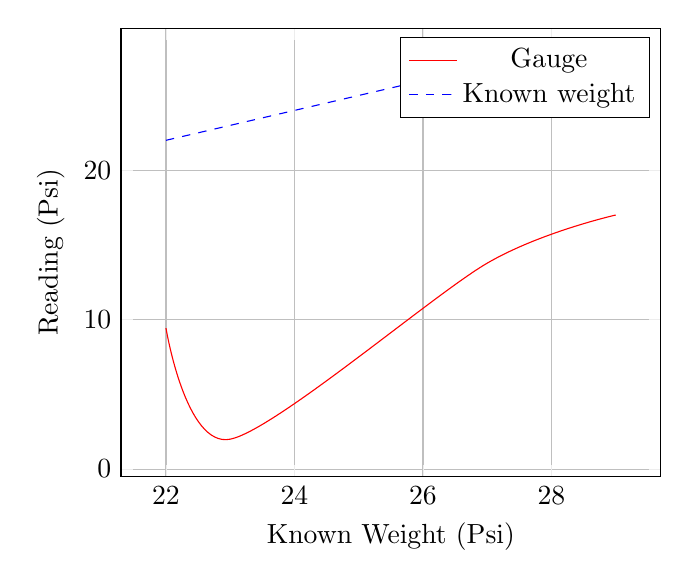
\begin{tikzpicture}
    \begin{axis}[
      xlabel=Known Weight (Psi),
      ylabel=Reading (Psi),
      grid=major]
    \addplot[color=red, smooth] coordinates {
      (22,9.43)
      (23, 2)
      (27,13.78)
      (29,17)
    };
    \addlegendentry{Gauge}
    
    \addplot[color=blue, dashed, smooth] coordinates {
      (22,22)
      (27,27)
    };
    \addlegendentry{Known weight}
    
    \end{axis}
  \end{tikzpicture}
  \caption{Dead weight tester and gauge measurements}
  \label{gaugePlot}
\end{figure}

\end{homeworkProblem}

\end{document}

%----------------------------------------------------------------------------------------
% INSTRUCTIONS AND TEMPLATE COMPONENTS
%----------------------------------------------------------------------------------------

% Document is structured in --> [document]
%                                 [homeworkProblem]
%                                   [homeworkSection]
%                                     [COMPONENTS]

% Set space - \vspace{length}
% Horizontal line - \hrule
% Pagebreak - \clearpage or \newpage - they seem to do the same thing

% Normal equation:
% \begin{equation}
%   p = \frac{p_g - k}{m}
% \end{equation}

% Aligned equation:
% \begin{equation}
%   \begin{split}
%     \rho_5  & = -\frac{\left(1575-1900\right)}{g\left(105\e{-3}-70\e{-3}\right)}\\
%             & = 946.56 \text{ kg/m\(^{-3}\)}\\
%     \rho_6  & = -\frac{\left(1900-2150\right)}{g\left(70\e{-3}-42\e{-3}\right)}\\
%             & = 910.15 \text{ kg/m\(^{-3}\)}\\
%   \end{split}
% \end{equation}

% Table: Can get from the table site!
% \begin{table}[h]
% \centering
% \begin{tabular}{cccc}
% \multicolumn{4}{c}{\cellcolor[HTML]{EFEFEF}DATA MEASUREMENTS} \\ \hline
% \multicolumn{1}{c|}{\begin{tabular}[c]{@{}c@{}}Known Weight \\ Pressure (Psi)\end{tabular}} & \multicolumn{1}{c|}{\begin{tabular}[c]{@{}c@{}}Known Weight\\ Pressure (Bar)\end{tabular}} & \multicolumn{1}{c|}{\begin{tabular}[c]{@{}c@{}}Gauge Pressure\\ (Psi)\end{tabular}} & \begin{tabular}[c]{@{}c@{}}Gauge Pressure\\ (Bar)\end{tabular} \\ \hline
% \multicolumn{1}{c|}{22} & \multicolumn{1}{c|}{1.52} & \multicolumn{1}{c|}{9.43} & 0.65 \\
% \multicolumn{1}{c|}{\textbf{27}} & \multicolumn{1}{c|}{\textbf{1.86}} & \multicolumn{1}{c|}{\textbf{13.78}} & \textbf{0.95} \\
% \multicolumn{1}{c|}{32} & \multicolumn{1}{c|}{2.21} & \multicolumn{1}{c|}{17.40} & 1.20 \\
% \multicolumn{1}{c|}{37} & \multicolumn{1}{c|}{2.55} & \multicolumn{1}{c|}{21.76} & 1.50 \\
% \multicolumn{1}{c|}{42} & \multicolumn{1}{c|}{2.90} & \multicolumn{1}{c|}{26.11} & 1.80 \\
% \multicolumn{1}{c|}{47} & \multicolumn{1}{c|}{3.24} & \multicolumn{1}{c|}{29.01} & 2.00 \\
% \multicolumn{1}{c|}{\textbf{52}} & \multicolumn{1}{c|}{\textbf{3.59}} & \multicolumn{1}{c|}{\textbf{33.36}} & \textbf{2.30} \\
% \multicolumn{1}{c|}{57} & \multicolumn{1}{c|}{3.93} & \multicolumn{1}{c|}{37.71} & 2.60 \\ \hline
% \end{tabular}
% \caption{Dead weight tester and gauge measurements}
% \label{gaugeMeasurements}
% \end{table}

% Picture:
% \begin{figure}[H]
%   \begin{center}
%     \includegraphics[width=0.4\columnwidth]{MEC2022SLab1Exp1}
%     \caption{Apparatus}
%     \label{liquidDiagram}
%   \end{center}
% \end{figure}

% Graph:
% \begin{figure}[H]
%   \centering
%   \begin{tikzpicture}
%     \begin{axis}[
%       xlabel=Known Weight (Psi),
%       ylabel=Reading (Psi),
%       grid=major]
%     \addplot[color=red, smooth] coordinates {
%       (22,9.43)
%       (27,13.78)
%     };
%     \addlegendentry{Gauge}
    
%     \addplot[color=blue, dashed, smooth] coordinates {
%       (22,22)
%       (27,27)
%     };
%     \addlegendentry{Known weight}
    
%     \end{axis}
%   \end{tikzpicture}
%   \caption{Dead weight tester and gauge measurements}
%   \label{gaugePlot}
% \end{figure}

% Indented Text: (bit of a hacky way to do it)
% \begin{quote}
% where \(p_g\) is the gauge reading, \(m\) is the error coefficient, \(p\) is the known (``correct'') pressure and \(k\) is the error constant
% \end{quote}

% Code Snippet:
% \begin{lstlisting}
% .model AKM02 D(Is=1.5n Rs=.5 Cjo=80p M=0.3 Vj=1 nbv=3 bv=6.2 Ibv=1m Vpk=6.2 mfg=OnSemi type=zener)
% \end{lstlisting}

% Bibliography:
% \begin{thebibliography}{99}
%   \bibitem{itemname}
%   Author,
%   Date.
%   \emph{Title}.
%   Edition.
%   Press.
%   \url{http://web.iitd.ac.in/~shouri/eel201/tuts/diode_switch.pdf}
% \end{thebibliography}
